\chapter{評価実験}
提案手法の有効性を示すため2種類の実験を行った。いずれもタスクの対象としてconnect4を扱っている。
一つ目の実験はコンピュータ同士の対戦データを用いて提案手法による想定図の妥当性の実証を試みた(以下データ実験と表記)。
二つ目の実験は自作のconnect4学習支援システムを用いて提案手法のユーザーインタフェースを含んだ優位性の実証を試みた(以下システム実験と表記)。
この章ではまず実験の際に用いたタスクであるconnect4と使用したモデルであるalphazero\_baselineについて述べる。そののちにデータ実験、システム実験の詳細と結果を記載する。
\section{connect4\cite{connect4}}
connect4はボードゲームの一種である。ルールは五目並べに極めて近く、二人のプレイヤーが交互に互いの駒を盤上に置き、最終的に縦・横・もしくは斜めに連続して4つの石を並べたプレイヤーの勝利となる。ただし、五目並べや連珠との相違点として「重力」の存在が挙げられる。
この「重力」とは各プレイヤーが石をボード上の最も下の行または既に置かれた石の上にしか置けないという規則を表している。そのため、各プレイヤーの選択肢はボードの列の数と等しい。
connect4の一般的なボードの広さは$6\times7$であり$6\times7$のコネクト4については1988年にAllis\cite{allis}により知識ベースの手法による先番勝利が証明された。
Tromp\cite{data}によるconnect4の$\alpha-\beta$木探索によって導かれた各盤面の最善手とそのデータも一般に公開されている。
また、connect4は盤上に全ての情報が開示されており、結果もどちらか一方の勝利または引き分けのみであるため2人ゼロ和完全情報ゲームに分類される。
本論文の実験において提案手法をconnect4に適用する際には最終盤面において4つ以上並んでいる石の座標を特徴として用いた。
\begin{figure}[t]
	\centering
	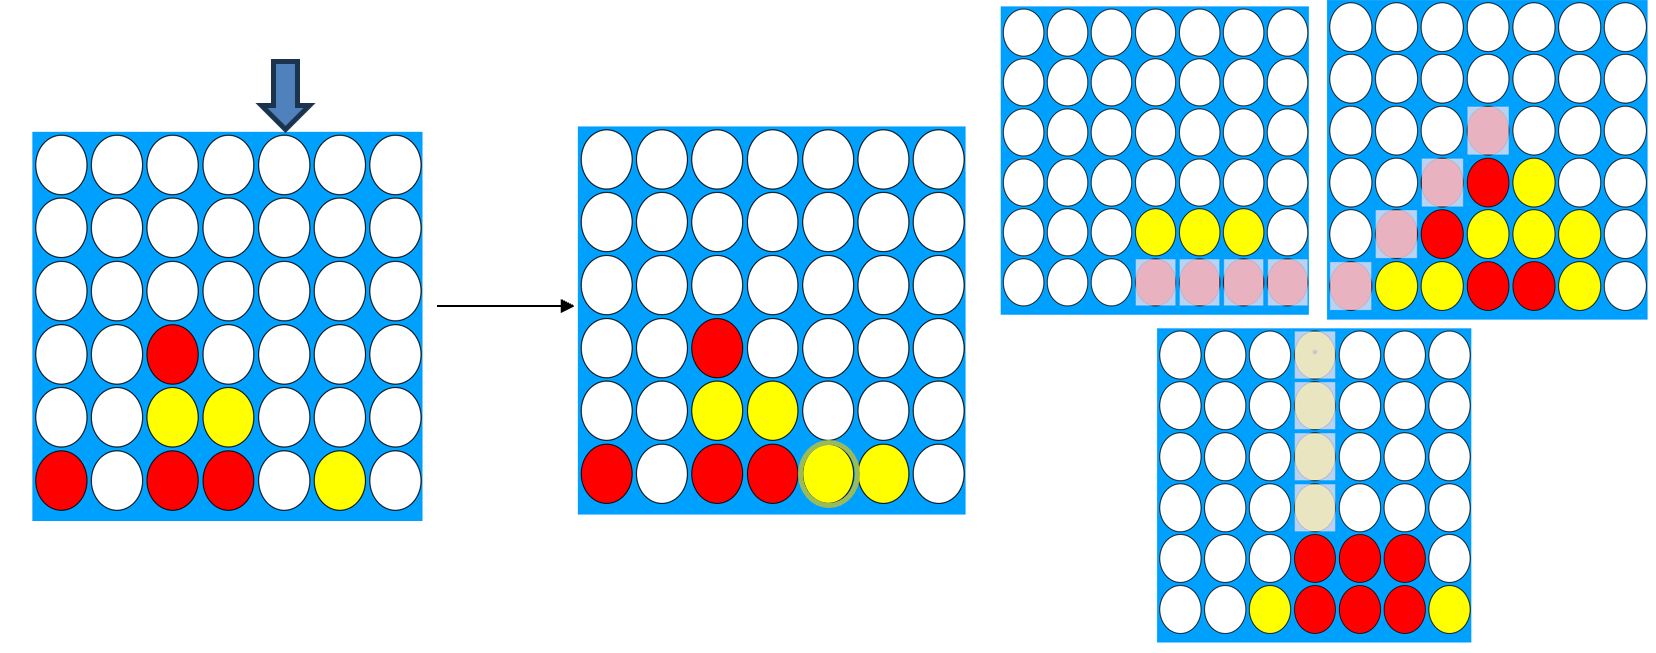
\includegraphics[width=\linewidth]{./figure/connect4.png}
	\caption{connect4}
	\label{fig:connect4}
\end{figure}
\section{alphazero\_baseline\cite{baseline}}
alphazero\_baselinはalphaZeroをconnect4用に簡易的に模したネットワークであり、入力は最新の盤面$s_0$、出力は$1\times7$(7はボードの列の数)の方策$P(s)(以下s=s_0とする)$とスカラー値の局面評価$V(s)$(値域は-1から1)である。
方策は確率分布であり、要素の値が大きいインデックスを選択することで勝利に近づくと予想される。
局面評価は入力に対する評価を表しており、1が入力の手番のプレイヤーにとっての勝利、-1が敗北の予想を表している。
\begin{figure}[t]
	\centering
	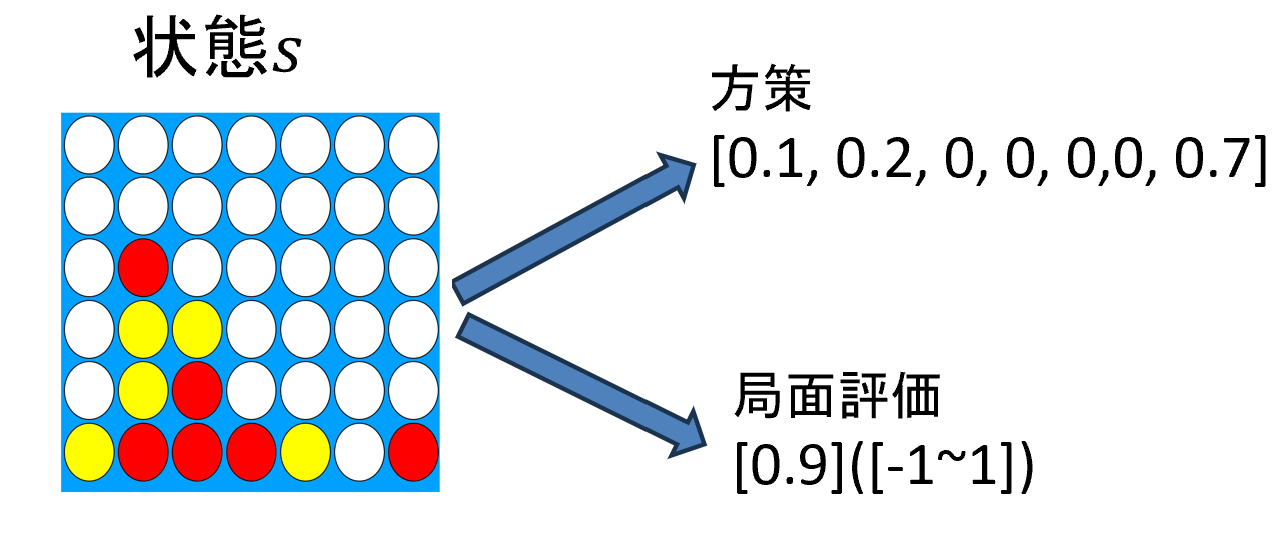
\includegraphics[width=\linewidth]{./figure/baseline.png}
	\caption{alphazero\_baselineの入出力}
	\label{fig:baseline}
\end{figure}

\section{データ実験}
\label{chap:evaluation}
提案手法と後に述べる比較手法によるゲーム結果(後で勝敗も含める)の予測精度を比較した。
\subsection{データセット}
alphazero\_baselinモデル同士の対戦データ2000局分(盤面数:61049)を使用した。いずれもいずれも弱いAIが先番のデータを使用している。これは弱いAIが後番の場合評価関数の変動が極めて小さくなることと、弱い側が先番を選択することが指導において一般的とされるためである。

\subsection{比較手法}
提案手法と比較手法はそれぞれ以下の方式で予測を行う。
比較手法の詳細なアルゴリズムは付録Bに記載した。
\begin{itemize}
	\item 比較手法: 探索の開始地点から最も訪問回数が大きい選択肢を選び、決定木の端までたどり着いた際にそこで四つ繋がっている石の組み合わせ、位置を記録する。
	\item 提案手法: 集めた盤面における4つ繋がっている石を集計し、出現頻度が高い4つの個別の石の位置と出現頻度が高い二つの組み合わせを記録する。組み合わせを二つ記録する理由は下の図のように最終的に繋がっている組み合わせが二つある可能性を考慮するためである。
\end{itemize}
図\ref{fig:compare}は比較手法の直感的なイメージを示している。
\begin{figure}[t]
	\centering
	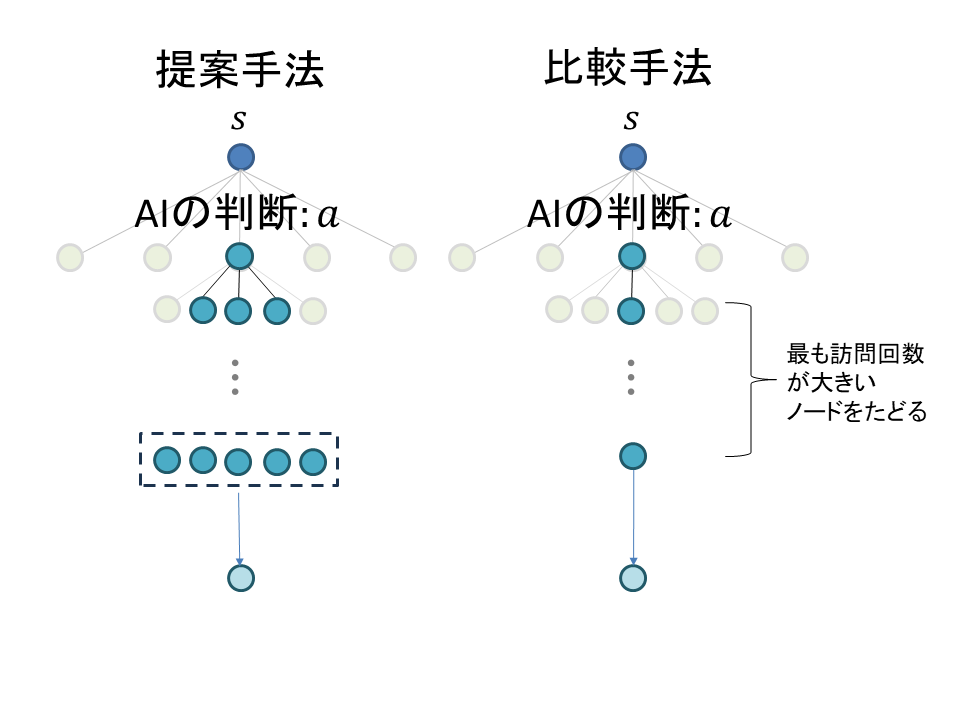
\includegraphics[width=\linewidth]{./figure/compare.png}
	\caption{提案手法と比較手法の比較}
	\label{fig:compare}
\end{figure}

\subsection{評価指標}
両手法による予測の精度を独自に定義した二つの定義group count($C_g$)、stone count($C_s$)によって計測した。stone count, group countの詳細な定義は付録Aに記載した。
どちらも最終盤面において4つ以上連続して並ぶ石と組み合わせ(以下fatal stone、fatal groupと記載)の座標に対する予測精度を表している。
ここでは概略を述べる。
手法によって予測されたfatal stone、fatal groupの座標をそれぞれ$F_s, F_g$とする。
\paragraph{group count}
予測の石の組み合わせ単位での精度を示しており、
手法による予測$F_g$と実際のfatal groupの集合$R_g$に共通する要素がある場合1、無い場合は1となる。
また、$F_g$と$R_g$が両方とも空集合$\phi$である場合(実際の結果が引き分けでありかつそれを正しく予測できている場合)group countは1となる。
\paragraph{stone count}
予測の個別の石単位での精度を表しており、
手法による予測$F_s$と実際の集合$R_s$の共通する要素の数を4で割った値である。値の最大値は1であり、先述の値が1を超える場合もstone countは1として扱う。
group countと同様に$F_s$と$R_s$が両方とも空集合である場合stone countは1となる。
\subsection{実験結果}


表\ref{table:result-online}に実験結果を示した。いずれの場合もgroup countにおいて提案手法は比較手法より高い値を示した。
表中に記載した「補間」の詳細は付録Bに記載した。
\begin{table}[H]
	\caption{実験結果:データ実験}
	\centering
	\scalebox{0.98}[0.98]{
		\begin{tabular}{c|c|c|c|c}
			\multicolumn{1}{c}{} & \multicolumn{2}{|c|}{group count} 
			& \multicolumn{2}{c|}{stone count}\\ \hline \hline
			手数(盤面数, 補間の有無)    & 提案手法 & 比較手法 & 提案手法 & 比較手法 \\ \hline
			19-24(9862, 無)    & \bf{0.60} & 0.43 & 0.55 & \bf{0.62} \\
			19-24(9862, 有)    & \bf{0.63} & 0.44 & 0.61 & \bf{0.63}  \\
			13-24(21022, 無)   & \bf{0.52} & 0.37 & 0.55 & \bf{0.56}  \\
			13-24(21022, 有)   & \bf{0.55} & 0.37 & 0.55 & \bf{0.56}  \\
		\end{tabular}
	}
	\label{table:result-online}
\end{table}
\section{システム実験}
提案手法の人間に対する有効性を示すため以下のような自作したconnect4の学習支援システムを用いて実験を行った。
実験対象者は計22人の10代-20代学生(男性17名:女性5名)となった。
\begin{figure}[t]
	\centering
	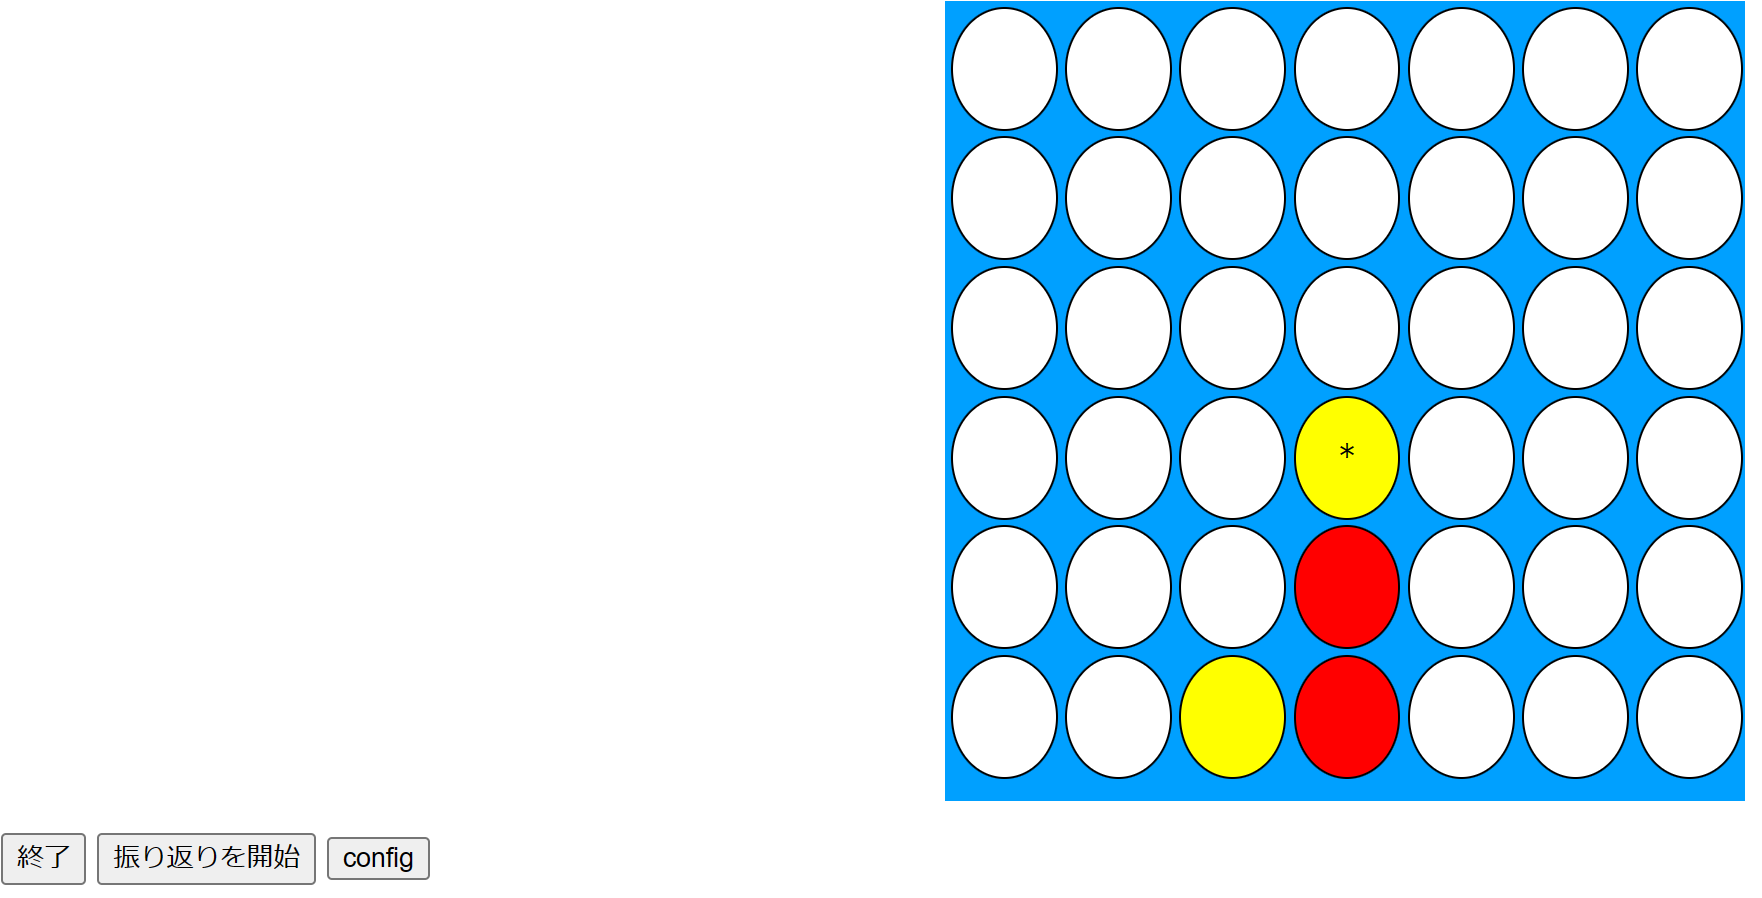
\includegraphics[width=\linewidth]{./figure/basicSystem.png}
	\caption{開始画面}
	\label{fig:basic}
\end{figure}
\subsection{実験手順}
実験は被験者一人あたりにつき三回行われ、前半二回を第一段階(提案手法による学習)、後半一回が第二段階(被験者同士の対戦)とした。
ここでは第一段階である提案手法の学習について述べる。
\paragraph{第一段階(提案手法による学習)}
提案システムを用いた学習はさらに
\begin{itemize}
	\item AIシステム(alphazero\_baseline)との対戦
	\item 提案手法によるゲームの振り返り
\end{itemize}
の2ステップに分けられる。AIシステムとの対戦が終了するとシステムは「振り返りモード」に移行する。
ユーザーはゲームの任意の地点において提案手法または比較手法が提案する予想図を見ることができる。
実験の際には被験者をグループA(提案手法による予想図を見せるグループ)とグループB(比較手法による予想図を見せるグループ)に分類した。
\begin{figure}[t]
	\centering
	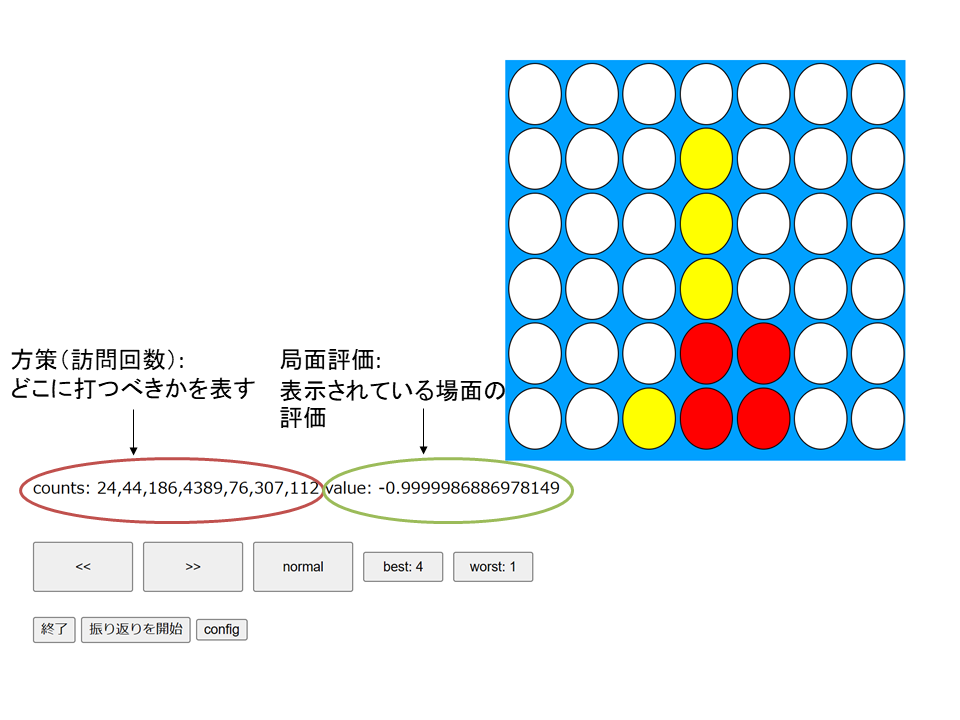
\includegraphics[width=\linewidth]{./figure/lookBack.png}
	\caption{振り返り画面}
	\label{fig:lookBack}
\end{figure}
数字が描かれたボタンは列のインデックスを表しており、各ボタンを押した際にその列を選択した場合の想定図と局面評価を確認できる。
\begin{figure}[t]
	\centering
	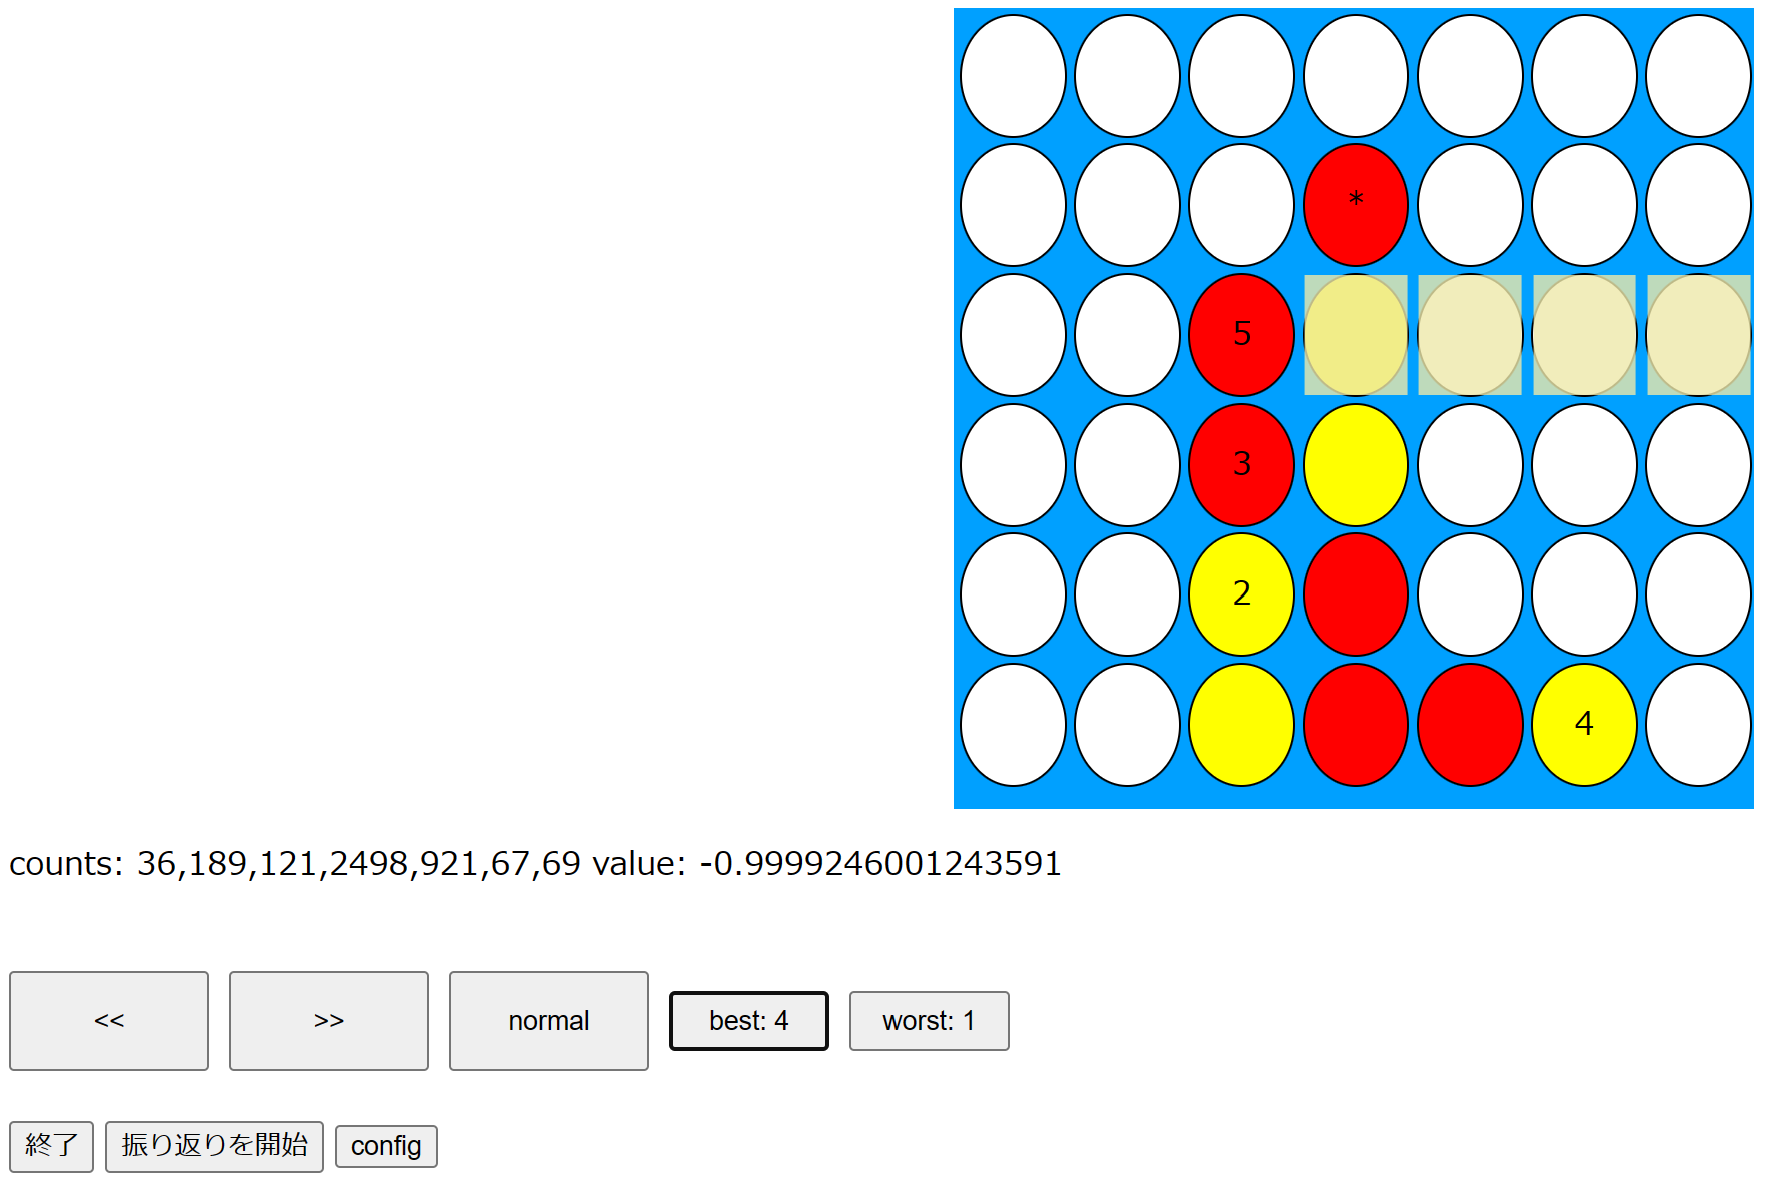
\includegraphics[width=\linewidth]{./figure/trajSystem.png}
	\caption{予想図の表示}
	\label{fig:trajSystem}
\end{figure}
\subsection{評価指標}
システム実験の評価指標は主観評価と客観評価の二つに分けられる。
主観評価は被験者による五段階評価であり、「タスクの熟達度に関連する質問」((a))と「タスクの楽しさ・面白さに関連する質問」((b))の二つに分けられる。
具体的な質問事項は付録Dに記載する。
客観評価はグループA(提案手法)の被験者とグループB(比較手法)の被験者の対戦成績である。

\subsection{実験結果}
予想図で提示される先読みの手数ごとに主観評価の平均値($1\sim5$)を表\ref{table:system-3}に示した。
先読み手数が3手または先読み手数制限なしの場合に、提案手法は比較手法に対して高い結果を示した。
\begin{table}[H]
    \caption{先読み手数3手の場合}
    \scriptsize
    \centering
    \resizebox{\linewidth}{!}{
        \begin{tabular}{c|l||c|c}
            \multicolumn{2}{c}{質問} & \multicolumn{2}{|c}{主観評価} \\ \hline \hline
            質問の種類 & 質問の内容 & A & B \\ \hline 
            (a) & 振り返りによって成長したと感じましたか & \bf{3.29} & 3.17 \\
            & 振り返りによってAIの意図を掴むことができたと感じますか & 2.43 & \bf{2.67} \\
            & (二回目のみ) 一回目に比べて成長したと感じますか & 2.75 & \bf{4.33} \\ \hline
            (b) & 今後も connect4 をプレイするときにこのシステムを使いたいと思いましたか & \bf{3.71} & 3.67 \\
            & システムにより振り返りが楽しくなったと感じますか & \bf{3.57} & 3.00 \\
        \end{tabular}
    }
    \label{table:system-3}
\end{table}
\begin{table}[H]
    \caption{先読み手数5手の場合}
    \scriptsize
    \centering
    \resizebox{\linewidth}{!}{
        \begin{tabular}{c|l||c|c}
            \multicolumn{2}{c}{質問} & \multicolumn{2}{|c}{主観評価} \\ \hline \hline
            質問の種類 & 質問の内容 & A & B \\ \hline 
            (a) & 振り返りによって成長したと感じましたか & 3.00 & \bf{4.00} \\
            & 振り返りによってAIの意図を掴むことができたと感じますか & 2.60 & \bf{4.00} \\
            & (二回目のみ) 一回目に比べて成長したと感じますか & 3.67 & \bf{4.33} \\ \hline
            (b) & 今後も connect4 をプレイするときにこのシステムを使いたいと思いましたか & 4.00 & \bf{4.80} \\
            & システムにより振り返りが楽しくなったと感じますか & 4.20 & \bf{4.60} \\
        \end{tabular}
    }
    \label{table:system-5}
\end{table}
\begin{table}[H]
    \caption{先読み手数7手の場合}
    \scriptsize
    \centering
    \resizebox{\linewidth}{!}{
        \begin{tabular}{c|l||c|c}
            \multicolumn{2}{c}{質問} & \multicolumn{2}{|c}{主観評価} \\ \hline \hline
            質問の種類 & 質問の内容 & A & B \\ \hline 
            (a) & 振り返りによって成長したと感じましたか & {3.83} & \bf{4.33} \\
            & 振り返りによってAIの意図を掴むことができたと感じますか & 2.67 & \bf{3.67} \\
            & (二回目のみ) 一回目に比べて成長したと感じますか & 2.75 & \bf{4.33} \\ \hline
            (b) & 今後も connect4 をプレイするときにこのシステムを使いたいと思いましたか & 4.17 & \bf{4.67} \\
            & システムにより振り返りが楽しくなったと感じますか & 3.00 & \bf{3.50} \\
        \end{tabular}
    }
    \label{table:system-7}
\end{table}
\begin{table}[H]
    \caption{先読み手数制限なしの場合}
    \scriptsize
    \centering
    \resizebox{\linewidth}{!}{
        \begin{tabular}{c|l||c|c}
            \multicolumn{2}{c}{質問} & \multicolumn{2}{|c}{主観評価} \\ \hline \hline
            質問の種類 & 質問の内容 & A & B \\ \hline 
            (a) & 振り返りによって成長したと感じましたか & \bf{4.25} & 4.00 \\
            & 振り返りによってAIの意図を掴むことができたと感じますか & \bf{3.50} & 3.00 \\
            & (二回目のみ) 一回目に比べて成長したと感じますか & 2.75 & \bf{4.33} \\ \hline
            (b) & 今後も connect4 をプレイするときにこのシステムを使いたいと思いましたか & \bf{4.5} & 4.00 \\
            & システムにより振り返りが楽しくなったと感じますか & \bf{4.75} & 4.40 \\
        \end{tabular}
    }
    \label{table:system-100}
\end{table}
また、第二段階である被験者同士の対戦結果は以下となった。
付録Dに示すように被験者一人に対して二回対戦を行った。結果として示すscoreは勝利を1,敗北を-1,引き分けを0
とした二回の対戦の平均値として定義される。
結果は表\ref{table:result-battle}に記載した。提案手法を用いて訓練を行ったグループ(A)は比較手法を用いて訓練を行ったグループ(B)よりも高い
勝率を記録した。
\begin{table}[H]
	\caption{対戦の結果}
	\centering
	\scalebox{0.98}[0.98]{
		\begin{tabular}{c|c}
			グループ & score \\ \hline
			A(提案手法)    & \bf{0.25} \\ 
			B(比較手法)    & -0.15 \\
		\end{tabular}
	}
	\label{table:result-battle}
\end{table}
\subsection{考察(システム実験)}




\begin{comment}
	また,ああああああ
\end{comment}

\begin{table}[H]
	\caption{あああといいいの予測誤差}
	\centering
	\scalebox{0.98}[0.98]{
		\begin{tabular}{c|c|c|c|c|c|c}
			\multicolumn{1}{c}{} & \multicolumn{2}{|c|}{2019} 
			& \multicolumn{2}{c|}{2018} & \multicolumn{2}{c}{2017}\\ \hline \hline
			モデル    & ああ & いい & ああ & いい & ああ & いい \\ \hline
			Naive    & \bf{1} & 1 & \bf{1} & 1 & \bf{1} & 1 \\
			TCN      & 1.0895 & 0.9032 & 1.4791 & \bf{0.9198} & 1.2888 & 0.8555 \\
			LSTM     & 1.0384 & 0.9295 & 1.4917 & 0.9725 & 1.1627 & 0.8541 \\
			提案手法  & 1.0977 & \bf{0.8698} & 1.3824 & 0.9439 & 1.2061 & \bf{0.8516} \\
		\end{tabular}
	}
	\label{table:result-2}
\end{table}
